%%% Econ712: Macroeconomics I
%%% Fall 2020
%%% Danny Edgel
%%%
% Due on Canvas Thursday November 12th, 11:59pm Central Time
%%%

%%%
%							PREAMBLE
%%%

\documentclass{article}

%%% declare packages
\usepackage{amsmath}
\usepackage{amssymb}
\usepackage{array}
\usepackage{bm}
\usepackage{changepage}
\usepackage{centernot}
\usepackage{graphicx}
\usepackage[shortlabels]{enumitem}
\usepackage{fancyhdr}
	\fancyhf{} % sets both header and footer to nothing
	\renewcommand{\headrulewidth}{0pt}
    \rfoot{Edgel, \thepage}
    \pagestyle{fancy}
	
%%% define shortcuts for set notation
\newcommand{\N}{\mathbb{N}}
\newcommand{\Z}{\mathbb{Z}}
\newcommand{\R}{\mathbb{R}}
\newcommand{\Q}{\mathbb{Q}}
\newcommand{\lmt}{\underset{x\rightarrow\infty}{\text{lim }}}
\newcommand{\neglmt}{\underset{x\rightarrow-\infty}{\text{lim }}}
\newcommand{\zerolmt}{\underset{x\rightarrow 0}{\text{lim }}}
\newcommand{\loge}[1]{\text{ln}\left(#1\right)}
\newcommand{\usmax}[1]{\underset{#1}{\text{max }}}
\newcommand{\Mt}{M_{t+1}^t}
\newcommand{\vhat}{\hat{v}}
\newcommand{\olp}{\overline{p}}
\renewcommand{\L}{\mathcal{L}}
\newcommand{\olq}{\overline{q}}

%%% define column vector command (from Michael Nattinger)
\newcount\colveccount
\newcommand*\colvec[1]{
        \global\colveccount#1
        \begin{pmatrix}
        \colvecnext
}
\def\colvecnext#1{
        #1
        \global\advance\colveccount-1
        \ifnum\colveccount>0
                \\
                \expandafter\colvecnext
        \else
                \end{pmatrix}
        \fi
}

%%% define function for drawing matrix augmentation lines
\newcommand\aug{\fboxsep=-\fboxrule\!\!\!\fbox{\strut}\!\!\!}

\makeatletter
\let\amsmath@bigm\bigm

\renewcommand{\bigm}[1]{%
  \ifcsname fenced@\string#1\endcsname
    \expandafter\@firstoftwo
  \else
    \expandafter\@secondoftwo
  \fi
  {\expandafter\amsmath@bigm\csname fenced@\string#1\endcsname}%
  {\amsmath@bigm#1}%
}


%________________________________________________________________%

\begin{document}

\title{	Problem Set \#1 }
\author{ 	Danny Edgel 					\\ 
			Econ 712: Macroeconomics I		\\
			Fall 2020						\\
		}
\maketitle\thispagestyle{empty}

%%%________________________________________________________________%%%

\noindent\textit{Collaborated with Sarah Bass, Emily Case, Michael Nattinger, and Alex Von Hafften}
\medskip \\

%%%________________________________________________________________%%%
\subsection*{Question 1}

\begin{enumerate}[(a)]
	\item The last period's consumption and current period's assets are taken as a given, while next period's consumption is chosen by selecting $A_{t+1}$. The Bellman equation for this problem, then, is:
		\[
			V(A) = \usmax{A'}\left\{u\left(\tilde{c},A-\frac{1}{R}A'\right) + \beta V(A')\right\}
		\]
		The feasible set for this problem is defined by the flow constraint, ${A_{t+1}\leq R(A_t - c_t)}$, and non-negativity constraint, ${A_{t+1}-RA_t\geq0}$. Thus, ${A'\in\Gamma[RA_t,R(A_t - c_t)]}$. In order to have a unique solution with a strictly increasing, strictly concave value function that is differentiable on the interior of the feasible set, the feasible set's domain must be convex, and the feasible set must be nonempty, compact-valued, and continuous. The function defining the feasible set must be monotone and convex. ${beta\in(0,1)}$, $u$ must be bounded and continuous, strictly increasing in $A'$ for all $A'$, and strictly convex and continuously differentiable over its domain.
		\medskip \\
		If the above conditions hold, then taking the first-order condition with respect to $A'$ yields:
		\[
			-\frac{1}{R}u'\left(\tilde{c},A-\frac{1}{R}A'\right) + \beta V'(A') = 0
		\]
		\begin{align*}
			\text{Envelope condition: } V'(A') &= u'\left(A-\frac{1}{R}A',A'-\frac{1}{R}A''\right) 	\\
			u'\left(A-\frac{1}{R}A',A'-\frac{1}{R}A''\right)  &= -\frac{1}{R}u'\left(A-\frac{1}{R}A',A'-\frac{1}{R}A''\right)+u'\left(A-\frac{1}{R}A',A'-\frac{1}{R}A''\right)	\\
			 &= \left(\frac{R-1}{R}\right)u'\left(A-\frac{1}{R}A',A'-\frac{1}{R}A''\right)
		\end{align*}
		Which results in the following condition for maximization:
		\[
			-\frac{1}{R}u'\left(\tilde{c},c\right) + \beta  \left(\frac{R-1}{R}\right)u'\left(g(c),g(c')\right) = 0
		\]
		Where $g(\cdot)$ is the optimal policy function.
	
	\item The optimal policy function is defined as
		\[
			c' = g(c) = \text{arg}\usmax{c'}\left\{\loge{c} + \gamma\loge{\tilde{c}} + \beta V(c')\right\}
		\]
		Which can be simplified as follows:
		\begin{align*}
			g(c) 	&= \text{arg}\usmax{c'}\left\{\beta V(c')\right\}	\\
			g(c) 	&= \text{arg}\usmax{c'}\left\{\beta \usmax{A''}\left\{  \loge{c'} + \gamma\loge{c} + \beta V(A'')\right\}\right\} 
		\end{align*}
		This maximization problem does not depend on $\tilde{c}$. Thus, the optimal saving policy is independent of past consumption. This can be shown also in the Bellman equation:
		\[
			V(A) = \usmax{A'}\left\{\loge{A-\frac{1}{R}A'} + \gamma\loge{\tilde{c}} + \beta V(A')\right\}= \gamma\loge{\tilde{c}}\usmax{A'}\left\{\loge{A-\frac{1}{R}A'} + \beta V(A')\right\}
		\]
		Taking the FOC of this problem and employing the envelope condition enables us to solve for the optimal savings policy function:
		\begin{align*}
			-\frac{1}{RA-A'} + \beta V'(A') &= 0	\\
			V'(A') &= \frac{1}{A'-\frac{1}{R}A''} - \frac{\gamma}{RA-A'}	\\
			\beta\left(\frac{1}{A'-\frac{1}{R}A''} - \frac{\gamma}{RA-A'}\right) &= \frac{1}{RA-A'}	\\
			\beta\left(\frac{RA-A'}{A'-\frac{1}{R}A''} -\gamma\right) &= 1 \\
			\frac{c}{c'} &= \frac{1+\beta\gamma}{R}
		\end{align*}
		Thus, the optimal policy is to save a constant traction of current assets.
		
	\item The result from (b) will not hold if we do not have a utility function that is seperable in $c_{t-1}$ and $c_t$. To see this, take ${u(c_{t-1},c_t)=c_{t-1}c_t}$. Using the maximization condition from part (a), the optimal policy function is:
		\begin{align*}
			-\tilde{c} + \beta(R-1)c' &= 0	\\
			c' &= \frac{\tilde{c}}{\beta(R-1)}
		\end{align*}
		This is clearly dependent on the last period's consumption and will thus not result in a constant fraction of current assets being chosen in each time period.
	
\end{enumerate}

%%%________________________________________________________________%%%
\subsection*{Question 2}

\begin{enumerate}[(a)]
	\item The sequential problem for the firm is:
		\[
			\usmax{\{x_t\}^\infty_{t=0}}\left\{ \delta^tF(x_t,x_{t+1}) \right\}
			=\usmax{\{x_t\}^\infty_{t=0}}\left\{ \delta^t\left(ax_t-\frac{1}{2}bx_t^2 - \frac{1}{2}c(x_{t+1}-x_t)^2\right) \right\}
		\]
		The Bellman equation is:
		\[
			V(x) = \usmax{x'}\left\{F(x,x') + \delta V(x')\right\} = 
			\usmax{x'}\left\{ ax-\frac{1}{2}bx^2 - \frac{1}{2}c(x'-x)^2 + \delta V(x') \right\}
		\]
		The maximization problem on the righthand side is a Bellman operator, $T$, defined as:
		\[
			(T)(v)(x) = \usmax{x'}ax-\frac{1}{2}bx^2 - \frac{1}{2}c(x'-x)^2 + \delta v(x')
		\]
	
	\item If we allow negative capital levels, then the domain of $x$ is $\R$. Then, for any value of $y$, ${ax-\frac{1}{2}bx^2 +\frac{1}{2}c(y-x)^2<ax}$, so $F$ has no lower bound. At the maximum value, $y-x=0$ in order to cancel the third term (which only subtracts from the other two terms). We can determine the maximum of the other two terms by taking first-order conditions, then plugging $\text{arg}\usmax{x,y}F(x,y)$ back into $F$:
		\begin{align*}
			a - bx &=0	\\
			x &= \frac{a}{b}	\\
			F\left(\frac{a}{b},\frac{a}{b}\right) &= a\left(\frac{a}{b}\right)-\frac{1}{2}b\left(\frac{a}{b}\right)^2 - \frac{1}{2}c\left(\left(\frac{a}{b}\right)-\left(\frac{a}{b}\right)\right)^2 = \frac{a^2}{b} - \frac{a^2}{2b}	\\
			F\left(\frac{a}{b},\frac{a}{b}\right) &= \frac{a^2}{2b}
		\end{align*}
		Since this upper bound of $F$ is achieved by ${x=\frac{a}{b}}$, which is a constant value, $\frac{a}{b}$ is the maximizer for the Bellman equation, which simplifies as:
		\begin{align*}
			V\left(\frac{a}{b}\right) =  \hat{v} &= F\left(\frac{a}{b},\frac{a}{b}\right) + \delta V\left(\frac{a}{b}\right)	\\
			(1-\delta)\hat{v}  &= \frac{a^2}{2b}	\\
			\hat{v}  &= \frac{a^2}{2b(1-\delta)}	\\
		\end{align*}
	
	\item Using the definition of $T$ provided in (a), we have:
		\begin{align*}
			(T\hat{v})(x) &= \usmax{x'}ax-\frac{1}{2}bx^2 - \frac{1}{2}c(x'-x)^2 + \delta \vhat	\\
			x'=x \Rightarrow (T\hat{v})(x) &= ax-\frac{1}{2}bx^2  + \delta \vhat
		\end{align*}
		Setting this weakly less than $\hat{v}$ gives:
		\begin{align*}
			T\hat{v}(x) &\leq \hat{v}	\\
			ax-\frac{1}{2}bx^2  + \delta \vhat  &\leq \frac{a^2}{2b(1-\delta)}	
		\end{align*}
		Which we showed as true in (b).
	
	\item \textit{Base step.} Let $n=1$. Then, let ${\alpha_1=a}$, ${\beta_1=b}$, and ${\gamma_1=\delta\vhat}$. In problem (c), we showed that this is the form taken by ${(T\vhat)(x)}$.
		\medskip \\
		\textit{Induction step.} Suppose that ${(T^n\vhat)(x) = \alpha_nx-\frac{1}{2}\beta_nx^2 + \gamma_n}$. Then,
		\begin{align*}
			(T^{n+1}\vhat)(x) 	&= T((T^n\vhat))(x)															\\
								&= \usmax{x'}ax-\frac{1}{2}bx^2 - \frac{1}{2}c(x'-x)^2 + \delta \left((T^n\vhat)(x)\right)	\\
			x'=x \Rightarrow (T^{n+1}\vhat)(x) &= ax-\frac{1}{2}bx^2  + \delta \left(\alpha_nx-\frac{1}{2}\beta_nx^2 + \gamma_n\right)	\\
								&= (a + \delta\alpha_n)x - \frac{1}{2}(b+\delta\beta_n)x^2 + \delta\gamma_n								\\
			(T^{n+1}\vhat)(x) 	&= \alpha_{n+1}x - \frac{1}{2}\beta_{n+1}x^2 + \gamma_{n+1}\text{ }\blacksquare
		\end{align*}
		Then, ${\alpha_{n+1} = a+\delta\alpha_n}$, ${\beta_{n+1} = b + \delta\beta_n}$, and ${\gamma_{n+1}=\delta\gamma_n}$
	
	\item As $n\rightarrow\infty$, $V(x)$ converges to:
		\begin{align*}
			V &= \underset{n\rightarrow\infty}{\text{lim }}(T^{n}\vhat)(x) 	\\
			V &= \underset{n\rightarrow\infty}{\text{lim }}\left\{ \alpha_{n+1}x - \frac{1}{2}\beta_{n+1}x^2 + \gamma_{n+1} \right\}	\\
			V &= a\left(\sum^n_{i=1}\delta^i\right)x - \frac{1}{2}b\left(\sum^n_{i=1}\delta^i\right)x^2 + \delta^n\vhat	\\
			V &= \left(\frac{a}{1-\delta}\right)x-\frac{1}{2}\left(\frac{b}{1-\delta}\right)x^2
		\end{align*}
		The image of $T$ at this $V$ is:
		\begin{align*}
			TV &= \usmax{x'}ax-\frac{1}{2}bx^2 - \frac{1}{2}c(x'-x)^2 + \delta V	\\
			x'=x \Rightarrow TV &= ax-\frac{1}{2}bx^2 + \delta \left(\frac{a}{1-\delta}\right)x-\frac{1}{2}\left(\frac{b}{1-\delta}\right)x^2	\\
			TV &= \left(a + \delta\frac{a}{1-\delta}\right)x-\frac{1}{2}\left(b + \delta\frac{b}{1-\delta}\right)x^2	\\
			TV &= \left(\frac{a}{1-\delta}\right)x-\frac{1}{2}\left(\frac{b}{1-\delta}\right)x^2	\\
			TV &= V
		\end{align*}
		Thus, the limit function satisfies the Bellman equation.
	
\end{enumerate}

%%%________________________________________________________________%%%
\subsection*{Question 3}

\begin{enumerate}[(a)]
	\item The Bellman equation for this problem is:
		\[
			V(k) = \usmax{k'}\left\{ \pi(k) - \gamma(k'-(1-\delta)k)+\frac{1}{R}V(k') \right\}
		\]
		The first-order condition of the right side of the Bellman provides the conditions for maximization:
		\begin{align*}
			-\gamma'(k'-(1-\delta)k)+\frac{1}{R}V'(k') &= 0	\\
			V'(k') &= \pi'(k') + (1-\delta)\gamma'(k''-(1-\delta)k')\text{ (envelope condition)}	\\
			R\gamma'(k'-(1-\delta)k) &= \pi'(k') + (1-\delta)\gamma'(k''-(1-\delta)k')
		\end{align*}
	
	\item A steady state in this system is a constant level of capital, ${\overline{k}=k=k'}$, and investment, ${\overline{I}=I=I'}$ such that the conditions for maximization are satisfied:
		\begin{align*}
			R\gamma'(\overline{I}) &= \pi'(\overline{k}) + (1-\delta)\gamma'(\overline{I})	\\
			\frac{\pi'(\overline{k})}{\gamma'(\overline{I})} &= R+\delta-1
		\end{align*}
		Given the convexity and continuity of the set of feasible values for $k$ and the fact that $\pi$ and $\gamma$ are both strictly increasing and continuous (thus making the objective function bounded), there exists a unique steady state solution.
		\smallskip \\
		An increase in $R$ would increase the ratio of marginal profit to marginal investment cost in the steady state. Since $\pi$ is strictly concave, marginal profit is strictly decreasing. Thus, an increase in the steady-state ratio of marginal profit to marginal investment cost is associated with a decrease in steady-state capital levels. Since $\overline{I}=\delta\overline{k}$, steady-state investment would also fall.
	
	\item The derivative of the profit and investment cost functions are:
		\[
			\pi'(k) = k-k^*\text{, } \gamma'(I) = I
		\]
		Thus, the relationship between investment and capital in the steady state is:
		\[
			\overline{k}(\overline{I}) = (R+\delta-1)\overline{I} + k^*
		\]
		This function represents the saddle path for each parameter $R$, $\delta$, and $k^*$. Plotting this at $R=1.05$ and $R=1.1$ against the resource constraint allows us to chart the movement of investment and capital following an exogenous shock to the interest rate:
		\begin{center}
			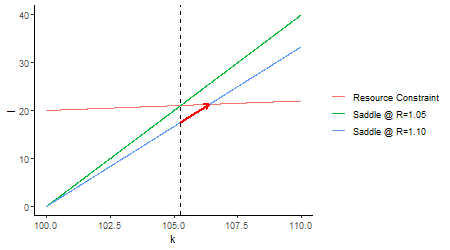
\includegraphics[scale=.7]{figure3c.png}
		\end{center}
	
\end{enumerate}

%%%________________________________________________________________%%%
\subsection*{Question 4}

\begin{enumerate}[(a)]
	\item 
	
	\item 
	
	\item 
	
\end{enumerate}

%%%________________________________________________________________%%%


\end{document}












